\documentclass[border=10pt]{standalone}

\usepackage{tikz}
\usepackage{tikzsymbols}
\usetikzlibrary{calc,patterns,shapes.geometric}

\def\centerarc[#1](#2)(#3:#4:#5){\draw[#1] ($(#2)+({#5*cos(#3)},{#5*sin(#3)})$) arc (#3:#4:#5);}

\begin{document}
	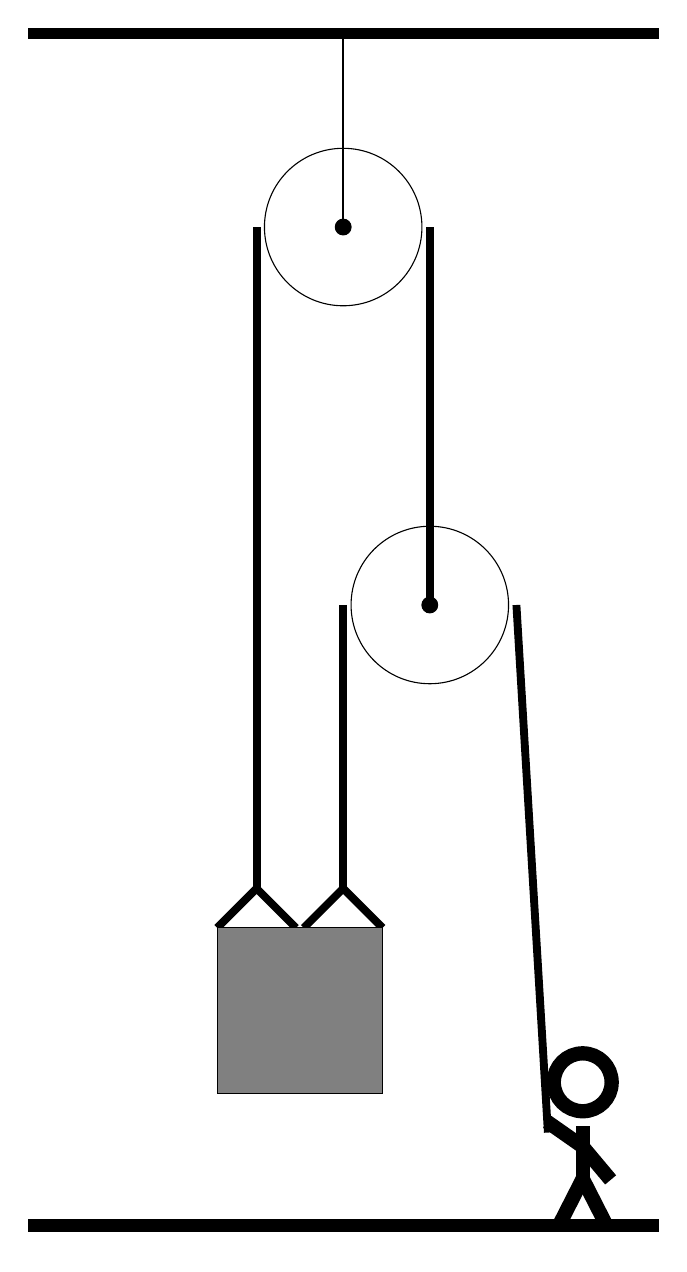
\begin{tikzpicture}
		%%%%% START %%%%%
		\draw[fill=black] (-2, 12) rectangle (6, 12.125);
		
		\draw (2, 9.6) circle (1);
		\draw[fill=black] (2, 9.6) circle (0.1);
		\draw[thick] (2, 9.6) -- (2, 12);
		
		\draw (3.1, 4.8) circle (1);
		\draw[fill=black] (3.1, 4.8) circle (0.1);
		
		\draw[line width = 1mm]  (0.4, 0.7) -- (0.9, 1.2) -- (1.4, 0.7);
		\draw[line width = 1mm]  (1.5, 0.7) -- (2.0, 1.2) -- (2.5, 0.7);
		\draw[fill=black!50] (0.4, 0.7) rectangle (2.5, -1.4);
		
		\draw[line width = 1mm] (0.9, 9.6) -- (0.9, 1.2);
		\centerarc[line width = 1mm](2, 9.6)(0:180:1.1);
		\draw[line width = 1mm] (3.1, 9.6) -- (3.1, 4.8);
		\draw[line width = 1mm] (2.0, 4.8) -- (2.0, 1.2);
		\centerarc[line width = 1mm](3.1, 4.8)(0:180:1.1);
		\draw[line width = 1mm] (4.2, 4.8) -- (4.6, -1.9);
		
		\node at (5, -2) {\Strichmaxerl[10][-35][-50]};
		
		\draw[fill=black] (-2, -3) rectangle (6, -3.15);
		%%%%% END %%%%%
	\end{tikzpicture}
\end{document}